\subsection{Корни из комплексных чисел}

$z^n = w,~n \in \N,~w \in \CC$

$w = 0 \implies z = 0$

$w \neq 0,~w = r (\cos \varphi + i \sin \varphi),~r > 0,~\varphi \in \R,~z = p (\cos \alpha + i \sin \alpha),~p > 0,~\alpha \in \R$

$z^n = w \iff p^n (\cos n \alpha + i \sin n \alpha) = r (\cos \varphi + i \sin \varphi) \iff$
$\begin{cases}
    p^n = r\\
    n \alpha = \varphi + 2 \pi k,~k \in \Z
\end{cases} \iff$

$\begin{cases}
    p = \sqrt[n]{r}\\
    \alpha = \frac{\varphi + 2 \pi k}{n},~k \in \Z
\end{cases}$

$z^n = w \iff z = \underbrace{\sqrt[n]{r} \left(\cos \frac{\varphi + 2 \pi k}{n} + i \sin \frac{\varphi + 2 \pi k}{n}\right)}_{z_k},~k \in \Z$

При каких $k, l: z_k = z_l$?

$z_k = z_l \iff \frac{\varphi + 2 \pi k}{n} = \frac{\varphi + 2 \pi l}{n} + 2 \pi s,~s \in \Z \iff \frac{k}{n} + \frac{l}{n} + s,~s \in \Z \iff $  

$k = l + ns,~s \in \Z \iff k \equivm{n} l \iff z \in \{z_0, z_1, \ldots, z_{n-1}\}$

Таким образом, мы доказали:

\begin{theorem}
    $\letus n \in \N,~w \in \CC$

    \begin{enumerate}
        \item Если $w = 0$, То уравнение $z^n = w$ имеет единственный корень $z = 0$.
        
        \item Если $w \neq 0$, То уравнение $z^n = w$ имеет ровно $n$ различных корней:
    
        \[ z_k = \sqrt[n]{r} \left(\cos \frac{\varphi + 2 \pi k}{n} + i \sin \frac{\varphi + 2 \pi k}{n}\right),~k = 0, 1, \ldots, n-1 \]

    \end{enumerate}
\end{theorem}

\subsubsection*{Изображение на окружности}

\begin{center}
    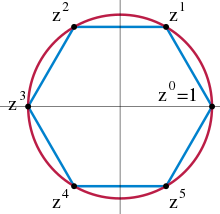
\includegraphics[width=0.3\textwidth]{images/complexroot.png}
\end{center}

Комплексные корни образуют праильный $n$-угольник на окружности.

\begin{lemma}
    Пусть $z_0, z_1, \ldots, z_{n - 1}$ --- все корни $z^n = w,~n > 1$

    Тогда $z_0 + z_1 + \ldots + z_{n - 1} = 0$
\end{lemma}

\begin{proof}

    $z_k = z_{k - 1} \underbrace{\left( \cos \frac{2 \pi}{n} + i \sin \frac{2 \pi}{n} \right)}_{\xi}$

    $S = z_0 + z_1 + \ldots + z_{n - 1}$

    $z_k = z_0 \cdot \xi^k$

    $\xi \cdot S = z_1 + z_2 + \ldots + \underbrace{z_n}_{= z_0} = S \implies (\xi - 1) S = 0$

    $n \neq 1 \implies \xi \neq 1$ 
    
    $(\xi - 1)S = 0 \implies S = 0$
\end{proof}

\begin{defn}
    Группа --- это множество $G$ с операцией $*: G \times G \to G$ такая, что:
    
    \begin{enumerate}
        \item $*$ --- ассоциативна: $(a * b) * c = a * (b * c)$
        \item Существует нейтраальный элемент $e \in G$ такой, что $a * e = e * a = a$ для любого $a \in G$
        \item У любого элемента $a \in G$ существует обратный элемент $a^{-1} \in G$ такой, что $a~*~a^{-1} = a^{-1} * a = e$
    \end{enumerate}
\end{defn}

\begin{examples}~

    \begin{enumerate}
        \item $(\Z, +)$
        \item $((\Z/n\Z)^*, \cdot)$
        \item Если $R$ --- ассоциативное кольцо с $1$, то $R^* = \{r \mid \exists s \in R : rs = sr = 1\}$ --- группа относительно умножения.
    \end{enumerate}
\end{examples}

Проверить замкнутость относительно умножения. 

Зафиксируем $n \in \N$

$\mu_n = \{ z \in \CC \mid z^n = 1\} = \{ \underbrace{\cos \frac{2 \pi k}{n} + i \sin \frac{2 \pi k}{n}}_{\xi_k} \mid k = 0, 1, \ldots, n-1 \}$ --- группа относительно умножения

$z, w \in \mu_n \implies zw \in \mu_n$ --- замкнутость относительно умножения

$(zw)^n = z^n w^n = 1 \cdot 1 = 1$

Доказательство, что $\mu_n$ --- группа:

\begin{itemize}
    \item Ассоциативность --- так как есть ассоциативность в $\CC$
    
    \item $1 \in \mu_n~(1 = \xi_0)$
    
    \item $\xi_k \cdot \xi_{-k} = \left( \cos \frac{2 \pi k}{n} + i \sin \frac{2 \pi k}{n} \right) \left( \cos \frac{2 \pi (-k)}{n} + i \sin \frac{2 \pi (-k)}{n} \right) = 1$
\end{itemize}

\begin{lemma}
    $\xi_k = \xi_1^k$
\end{lemma}

\begin{proof}
    $\left(1 \cdot \cos \frac{2 \pi k}{n} + i \sin \frac{2 \pi}{n}\right)^k = 1 \cdot \left( \cos \frac{2 \pi k}{n} + i \sin \frac{2 \pi k}{n} \right)$ (по формуле Муавра)
\end{proof}

\begin{defn}
    $G$ --- группа с операцией $*$, $g \in G,~n \in \Z$\\

    $g^n = \begin{cases}
        g~*~g~*~\ldots~*~g & n > 0 \\
        e & n = 0 \\
        g^{-1} * g^{-1} *~\ldots~* g^{-1} & n < 0
    \end{cases}$
\end{defn}

\begin{defn}
    Группа $G$ называется циклической, если $\exists g \in G : G = \{g^n \mid n \in \Z\}$

    Пишут: $G = \langle g \rangle$
\end{defn}

\begin{defn}
    $g$ --- образующий элемент группы $G$
\end{defn}

\begin{examples}~
    
    \begin{itemize}
        \item $\Z = \langle 1 \rangle = \langle -1 \rangle$ (по сложению) $g^n = \begin{cases}
            1 + 1 + \ldots + 1 & n > 0 \\
            0 & n = 0 \\
            -1 + -1 + \ldots + -1 & n < 0
        \end{cases}$

        \item $\Z/5\Z = \langle \oln{1} \rangle = \langle \oln{2} \rangle = \langle \oln{3} \rangle = \langle \oln{4} \rangle$ (по сложению)
        
        \item $\Z/6\Z = \langle \oln{1} \rangle = \langle \oln{5} \rangle$ (по сложению)
        
        \item $(\Z/5\Z)^* = \langle \oln{2} \rangle = \langle \oln{3} \rangle$ (по умножению)
        
        \item $(\Z/8\Z)^*$ --- не циклическая группа $g^2 = e \implies g^{2k} = e,~g^{2k+1} = g$
    \end{itemize}
\end{examples}

\begin{defn}
    $G$ --- группа, $g \in G$

    Если $\forall n \in \N: g^n \neq e$, то говорят, что $g$ --- бесконечный порядок

    Если $\exists n \in \N: g^n = e$, то минимальное такое $n$ называют порядком $g$ (пишут: $\ord g = n$)
\end{defn}

\begin{example}
    $\Z/5\Z$

    $\ord \oln{1} = 1$

    $\ord \oln{2} = 4$
    
    $\ord \oln{3} = 4$
    
    $\ord \oln{4} = 2$
\end{example}

\begin{theorem-non}
    Пусть $G$ --- конечная группа, $|G| = n,~g \in G$.

    Тогда: $G = \langle g \rangle \iff \ord g = n$
\end{theorem-non}

\begin{proof}
    "$\Rightarrow$":

    $\exists k, l: g^k = g^l,~k, l \in \{0, 1, \ldots, n\},~k \neq l$ (так как $G$ конечная)

    $k < l$: $g^{-k} \cdot g^k = g^{-k} \cdot g^l = g^{l - k} = e$

    $0 < l - k \leq n$

    Таким образом, порядок $g$ не превосходит $n$

    Предположим, $\ord g = m < n$

    $G = \{ g^k \mid k \in \Z \} = \{ g^{mq + r} \mid q \in \Z,~0 \leq r < m \} = \{g^0, g^1, \ldots, g^{m-1}\}$ --- противоречие, так как $|G| \leq m < n$

    "$\Leftarrow$":

    $\ord g = n$

    $\implies g^0, g^1, g^2, \ldots, g^{n - 1}$ --- они попарно различны

    $\implies \{g^0, g^1, \ldots, g^{n - 1}\} = G$

    $\implies G = \langle g \rangle$
\end{proof}

\begin{defn}
    Первообразным корнем из $1$ степени $n$ называется такой элемент $z \in \CC^*$, что $\ord z = n$
\end{defn}

\begin{example}
    $\mu_6 = \{1, \xi_1, \xi_2, \xi_3, \xi_4, \xi_5\}$
    
    $\ord 1 = 1$, $\ord \xi_1 = 6$, $\ord \xi_2 = 3$, $\ord \xi_3 = 2$, $\ord \xi_4 = 3$, $\ord \xi_5 = 6$

    $\xi_2$ --- первообразный корень из $1$ степени $3$
\end{example}